% \documentclass{beamer}
\documentclass[xcolor=dvipsnames]{beamer}
\usefonttheme{serif}
%% \usecolortheme[named=Blue]{structure}
\setbeamersize{text margin left=30mm, text margin right=30mm}
\useoutertheme{infolines}
%% \usetheme[height=7mm]{Rochester}
\usetheme{Pittsburgh}
\setbeamertemplate{items}[ball]
\setbeamertemplate{blocks}[rounded][shadow=true]
\setbeamertemplate{navigation symbols}{}

\usepackage[utf8x]{inputenc}
%% \usepackage{default}
\usepackage[english]{babel}
\usepackage{geometry}
%% \usepackage{fullpage}
\usepackage{amsmath, amsthm, amssymb}
\usepackage{listings}
\usepackage{pxfonts}
\usepackage{caption}


\captionsetup[figure]{labelformat=empty}

%% \usepackage{color}
%% \usepackage{graphicx}
%% \usepackage{natbib}
%% \usepackage{array}
%% \usepackage{booktabs}
%% \usepackage{tabu}
%% \usepackage[utf8]{inputenc}
%% \usepackage{fancyhdr}
%% \usepackage{float}
%% \usepackage{subfigure}
%% \usepackage{titlesec}

\setbeamertemplate{headline}{}
\setbeamertemplate{footline}[frame number]{}
\setbeamertemplate{navigation symbols}{}
\setbeamertemplate{footline}{}
\setbeamertemplate{footline}[frame number]

\setbeamertemplate{itemize items}{$-$}

\def\CCT{{C\nolinebreak[4]\hspace{-.05em}\raisebox{.4ex}{\tiny\bf ++}}}
\def\CC{{C\nolinebreak[4]\hspace{-.05em}\raisebox{.4ex}{\small\bf ++}}}


\definecolor{lstgray}{gray}{0.93}
\definecolor{strgray}{gray}{0.4}

\lstset{ %
  escapechar=@,
  language=C++,
  basicstyle=\footnotesize\ttfamily,
  %% basicstyle=\ttfamily,
  %% keywordstyle=\color{blue}\ttfamily,
  keywordstyle=\bfseries,
  stringstyle=\color{strgray}\ttfamily,
  commentstyle=\color{OliveGreen}\ttfamily,
  %% morecomment=[l][\color{red}]{\#},
  morecomment=[l][\color{blue}]{\#},
  backgroundcolor=\color{lstgray},
  %% keywordstyle=\color{red},
  frame=f,
  frameround=ffff,
  tabsize=2,
  breaklines=true,
  breakatwhitespace=false,
  showspaces=false,
  showstringspaces=false,
  xleftmargin=5pt,
  xrightmargin=5pt,
  morekeywords={in,out,ref,auto,inout,import,ushort,scope,exit,mixin,decltype,varid,sizeof,constexpr}
}

\def\redcolor{\color{red}}
\def\bluecolor{\color{blue}}
\def\blackcolor{\color{black}}
\def\graycolor{\color{gray}}
\def\greencolor{\color{OliveGreen}}


\def\sectionname{\translate{Section}}
\def\insertsectionnumber{\arabic{section}}
\setbeamertemplate{section page}
{
  \begin{centering}
    \begin{beamercolorbox}[sep=4pt,center]{part title}
      \usebeamerfont{section title}\insertsection\par
    \end{beamercolorbox}
  \end{centering}
}
\def\sectionpage{\usebeamertemplate*{section page}}


\AtBeginSection{\frame{\sectionpage}}


\title{Universals}
\subtitle{(In the 21\textsuperscript{st} Century)}
\author{Dominic Jones}
\date{\small{August 2019}}
\institute{\small{University of Buckingham}}


\begin{document}


\begin{frame}[plain]
  \titlepage
\end{frame}


\begin{frame}[fragile]{General argument}
  \begin{itemize}
  \item I argue that unity, truth, and goodness are transcendental properties of being, whereas beauty is a \emph{derived} property from these three.\vspace{5mm}
  \item It is when \emph{we} see those three properties shining together in something, we call it \emph{beautiful}.\vspace{5mm}
  \item But to have some idea about transcendentals, first some ideas about \emph{particulars}, \emph{concepts} and \emph{universals} are would be helpful.
  \end{itemize}
\end{frame}


\begin{frame}[fragile]{This talk}
  \begin{itemize}
  \item Unity, truth and goodness are abstracted, but are not \emph{just} concepts.\vspace{5mm}
  \item \emph{(But beauty is more like a judgement from the union of concepts.)}\vspace{5mm}
  \item Agreement on what is beautiful is seldom universal. \vspace{5mm}
  \item \emph{(But agreement on unity, ((less so truth) and less so goodness) more readily found.)}\vspace{5mm}
  \end{itemize}
\end{frame}




\begin{frame}{The one and the many}
  \begin{quote}
    {It is not too much of an exaggeration to say that virtually every major religious, moral, and political controversy of the last several centuries in some way rests on a disagreement, even implicit and unnoticed, over the `problem of universals'.}
  \end{quote}
%% \vspace{10mm}
      \hspace*{8cm}{Edward Feser}
\end{frame}


\begin{frame}{A grounding problem}
\begin{figure}
  \centering
  \begin{columns}
    \column{0.5\textwidth}
    \centering
    \caption {There's marriage}
    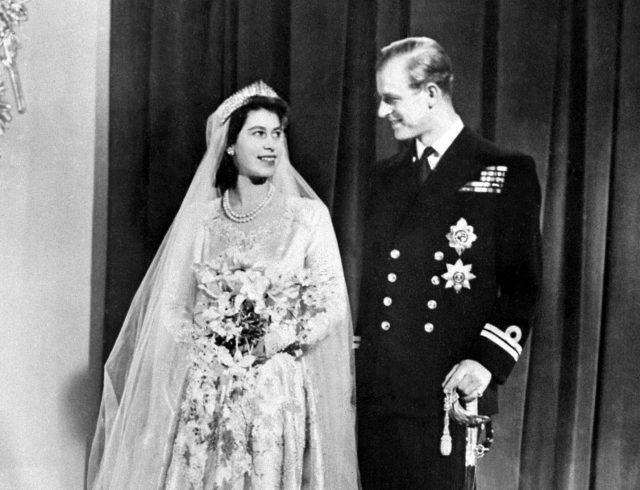
\includegraphics[width=0.99\textwidth]{conjugal}
    \column{0.5\textwidth}
    \centering
    \caption {{\ldots} and then there's marriage}
    \includegraphics[width=0.99\textwidth]{consentual}
  \end{columns}
\end{figure}
  Does the universal `marriage', for example, exist independently of finite minds?
\end{frame}


\begin{frame}{Realism}
  \begin{columns}
    \column{0.8\textwidth}
Realism affirms that universals --- `triangularity', `catness', etc., --- are irreducible to their particular instances and exist in a way that is in some sense independent of the human mind.
  \end{columns}
\end{frame}


\begin{frame}{Nominalism}
  \begin{columns}
    \column{0.8\textwidth}
Nominalism denies that there are any true universals and insists that only particulars are real --- there is this triangle and that one, this cat and that one, but no such thing as `triangularity' or `catness' over and above them.
  \end{columns}
\end{frame}


\begin{frame}{Conceptualism}
  \begin{columns}
    \column{0.8\textwidth}
Conceptualism holds that universals exist, but only in the mind --- `triangularity', `catness', etc., are the products of abstraction, and correspond to nothing in the world of external objects, all of which are particular.
  \end{columns}
\end{frame}


\begin{frame}{\emph{Knowledge argument}, Jackson 1986}
  \begin{figure}
    \centering
    
\includegraphics[width=0.6\textwidth]{mary-song}
    \caption {Upon seeing a red apple, does she know something new?}
  \end{figure}
\end{frame}


\begin{frame}{The abstract and the particular}
\begin{figure}
  \centering
  \begin{columns}
    \column{0.5\textwidth}
    \centering
    \caption {\emph{That which is triangular}}
    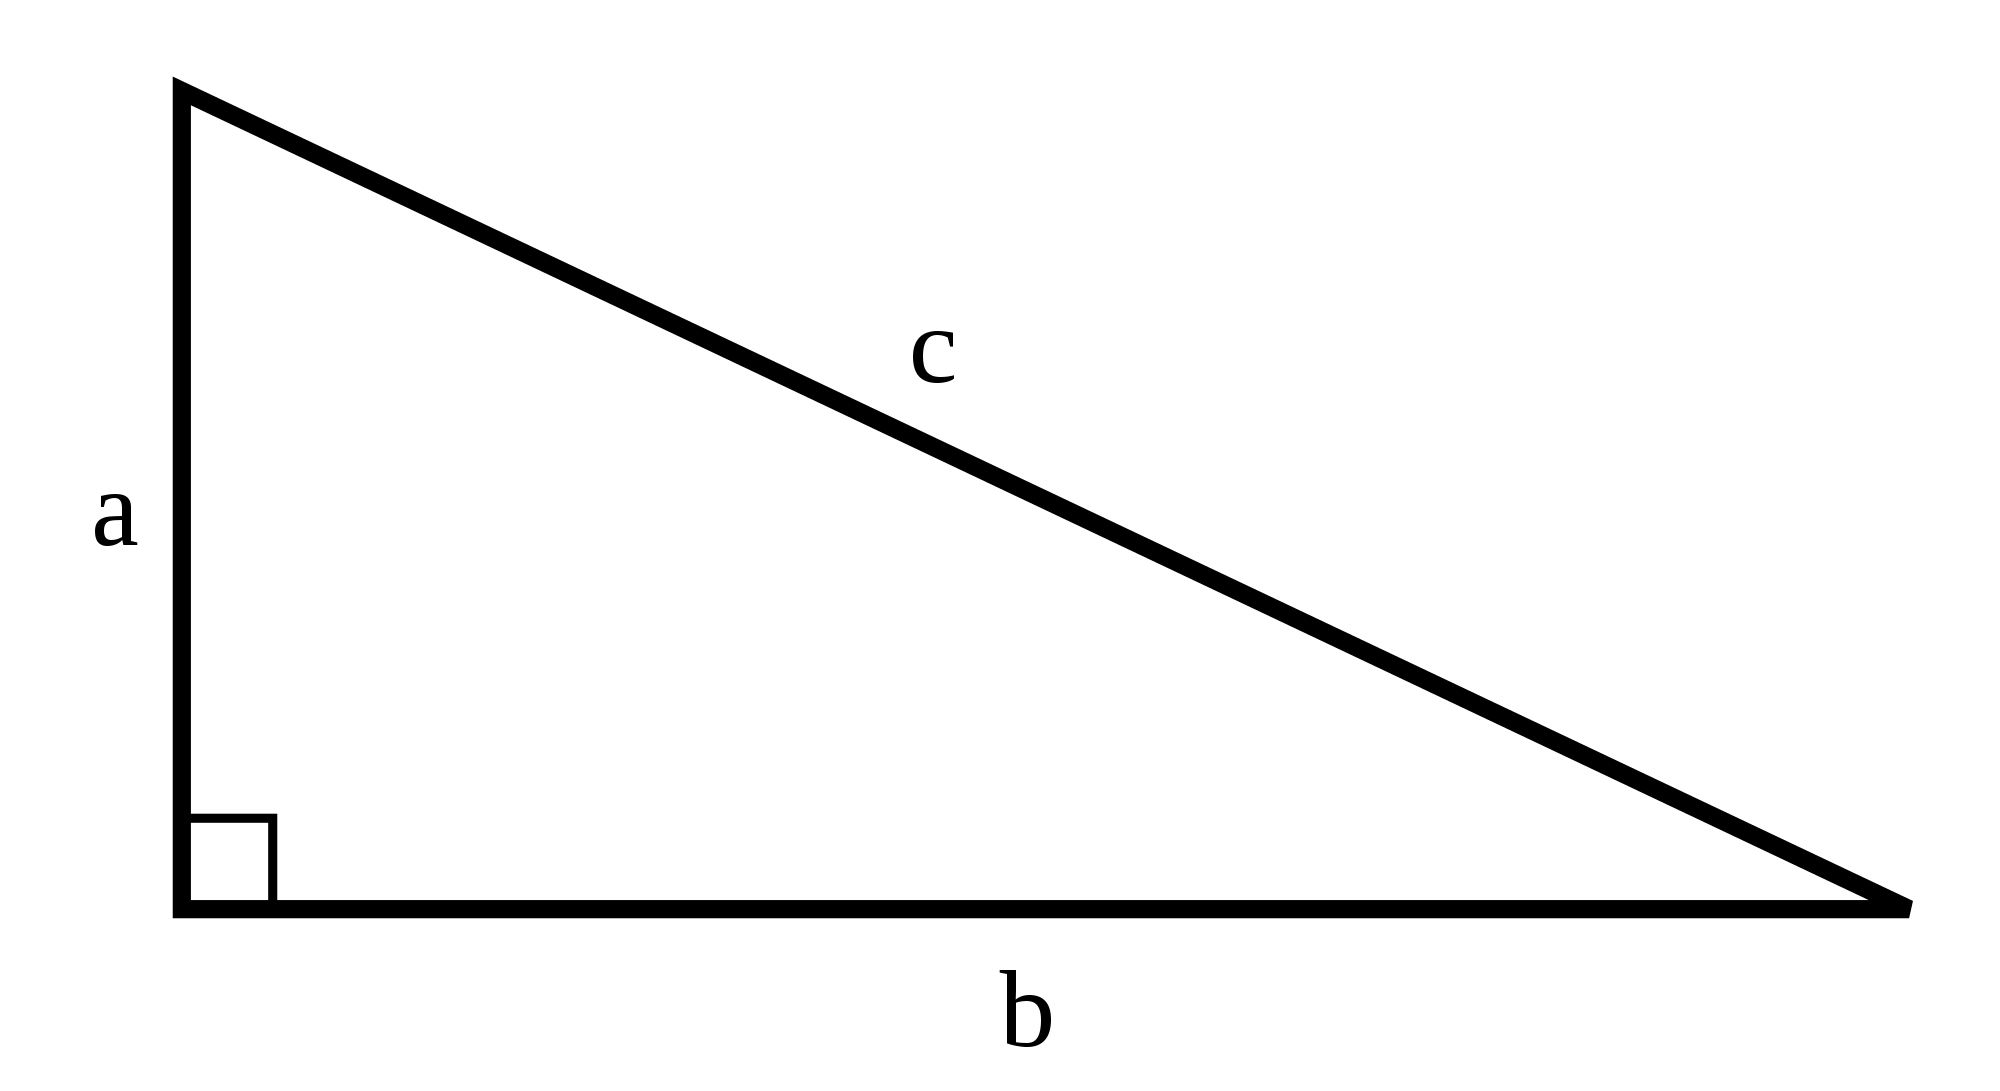
\includegraphics[width=0.99\textwidth]{triangular}
    \column{0.5\textwidth}
    \centering
    \caption {An imperfect instance}
    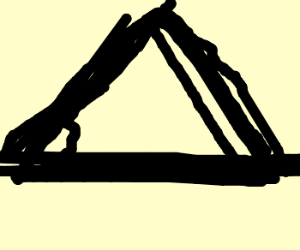
\includegraphics[width=0.99\textwidth]{triangle}
  \end{columns}
\end{figure}
I recognise something to be triangular, despite its imperfections.
\end{frame}


\begin{frame}{614-609mn monochromatic light}
\begin{figure}
  \centering
  \begin{columns}
    \column{0.5\textwidth}
    \centering
    \caption {A red thing}
    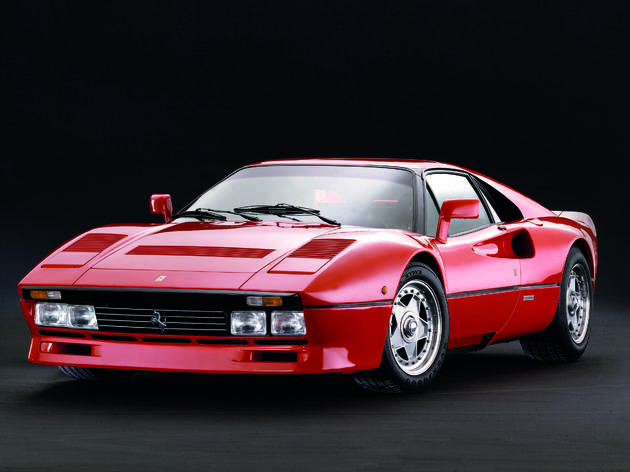
\includegraphics[width=0.99\textwidth]{ferrari}
    \column{0.5\textwidth}
    \centering
    \caption {Another red thing}
    
\includegraphics[width=0.99\textwidth]{red_sign}
  \end{columns}
\end{figure}
Not singular in spectrum, but still conceptually singular
\end{frame}


\begin{frame}{Distant cousins}
\begin{figure}
  \centering
  \begin{columns}
    \column{0.5\textwidth}
    \centering
    \caption {Non-rational}
    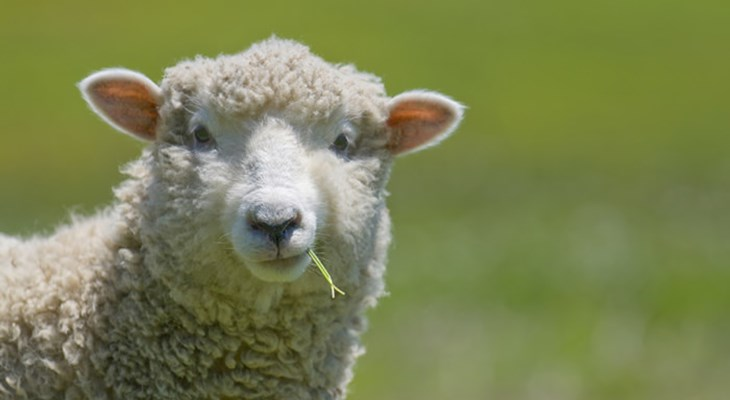
\includegraphics[width=0.99\textwidth]{sheep}
    \column{0.5\textwidth}
    \centering
    \caption {Rational}
    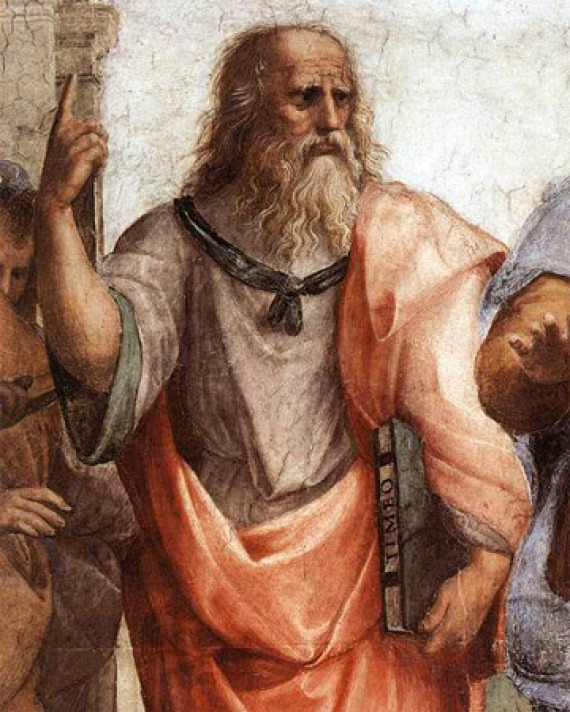
\includegraphics[width=0.6\textwidth]{plato}
  \end{columns}
\end{figure}
An individual animal is either rational or non-rational, but \emph{animality} entails neither.
\end{frame}


\begin{frame}{It couldn't be otherwise}
\begin{figure}
  \centering
  \begin{columns}
    \column{0.99\textwidth}
    \centering
    \caption {It is \emph{this concept} which is commonly known}
    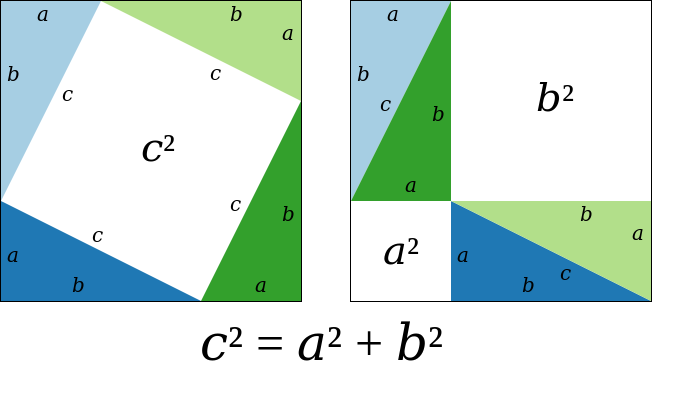
\includegraphics[width=0.8\textwidth]{pythagoras_proof}
  \end{columns}
\end{figure}
True prior to Pythagoras, and prior to matter.
\end{frame}



\begin{frame}{Platonic Realism}
  \begin{columns}
    \column{0.8\textwidth}
Universals exist in a `third realm' distinct from the world of particular things {and} distinct from the human mind.
  \end{columns}
\end{frame}


\begin{frame}{\emph{The Road to Reality}, Penrose 2004}
  \centering
  \begin{columns}
    \column{0.45\textwidth}
    \centering
    \begin{figure}
    \centering
    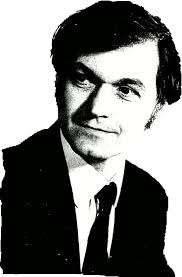
\includegraphics[width=0.7\textwidth]{r-penrose}
    %% \caption {\textbf{Clockwise}: mysteries,\;\; \textbf{Counter-clockwise}: prejudices}
  \end{figure}
    \column{0.6\textwidth}
    %% \centering
    %% \caption {Rational}
    %% 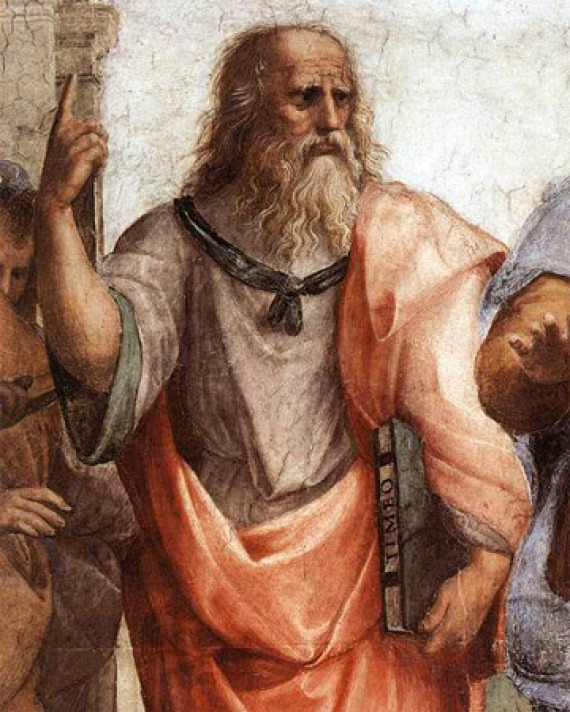
\includegraphics[width=0.6\textwidth]{plato}
    \textbf{Mysteries of the Third Realm}
    \begin{itemize}
\item Why do mathematical laws apply to the physical world with such precision?
\item How can some physical materials like human brains conjure up consciousness?
\item How is it that we can perceive mathematical truth?
    \end{itemize}
  \end{columns}
\end{frame}



\begin{frame}{\emph{The Road to Reality}, Penrose 2004}
  \centering
  \begin{columns}
    \column{0.45\textwidth}
    \centering
    \begin{figure}
    \centering
    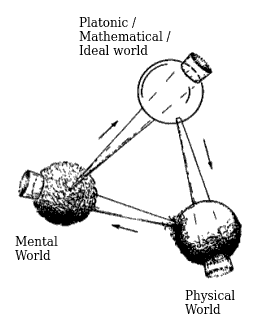
\includegraphics[width=0.99\textwidth]{penrose}
    %% \caption {\textbf{Clockwise}: mysteries,\;\; \textbf{Counter-clockwise}: prejudices}
  \end{figure}
    \column{0.6\textwidth}
    %% \centering
    %% \caption {Rational}
    %% 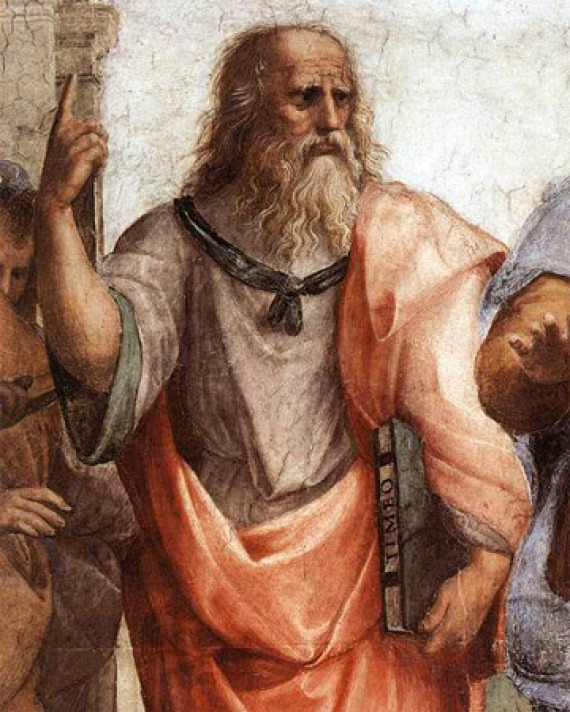
\includegraphics[width=0.6\textwidth]{plato}
    \textbf{Clockwise --- `mysteries'}
    \begin{itemize}
\item Part of the ideal is relevant to the physical
\item Part of the physical induces the mental
\item Part of the mental is concerned with the ideal
    \end{itemize}

\textbf{Counter-clockwise --- `prejudices'}
    \begin{itemize}
\item Possibility of mathematical truths inaccessible to reason
\item Possibility of mentality not rooted in physical structures
\item Possibility of physical action beyond the scope of mathematical control
    \end{itemize}
  \end{columns}
\end{frame}


\begin{frame}{Aristotelian Realism}
  \begin{columns}
    \column{0.8\textwidth}
Universals exist {only} in the particular things that instantiate them and in the intellect that abstracts them from from the particulars.
  \end{columns}
\end{frame}


\begin{frame}{From apples to the concept of `apple'}
\begin{figure}
  \centering
  \begin{columns}
    \column{0.99\textwidth}
    \centering
    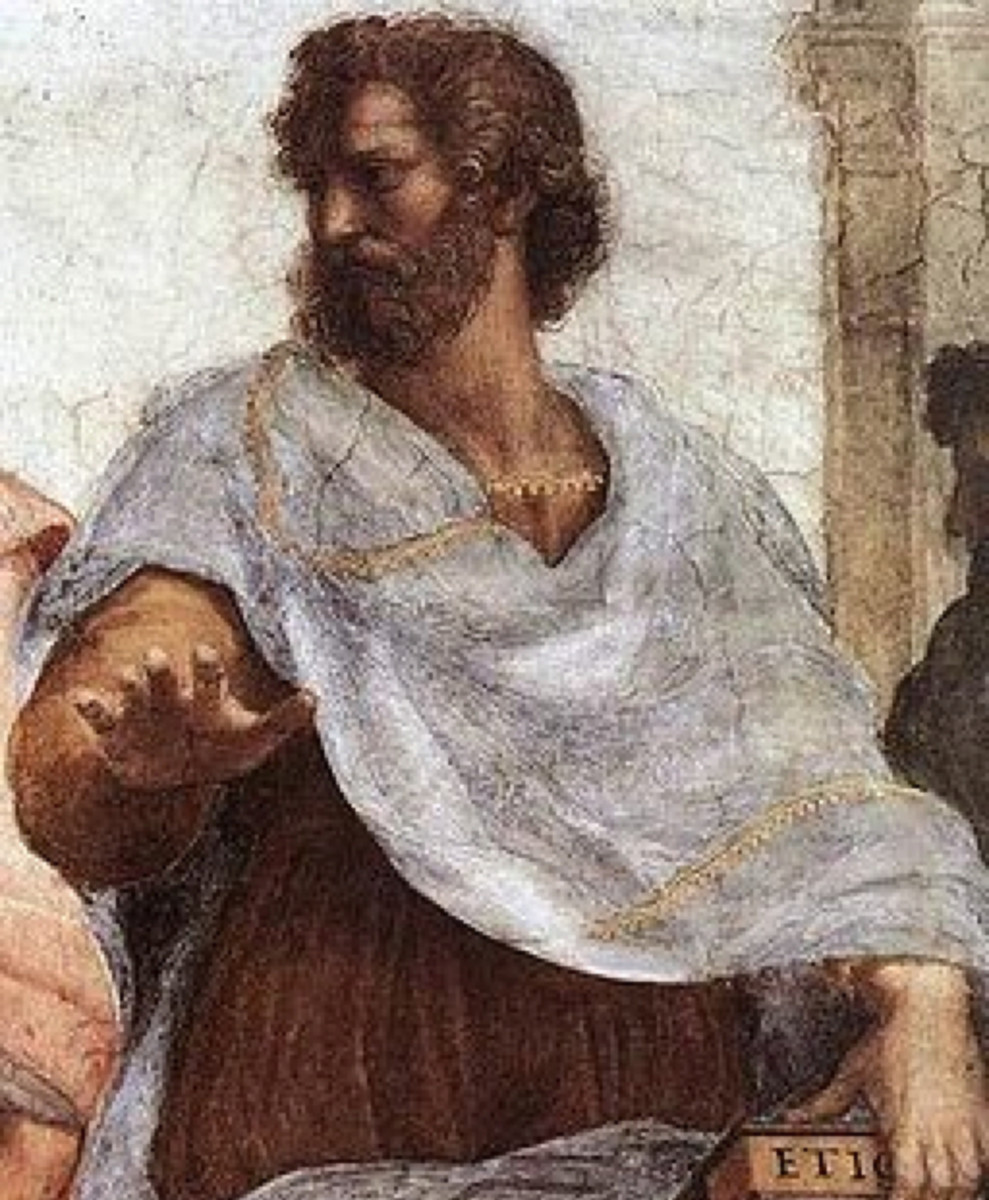
\includegraphics[width=0.5\textwidth]{aristotle}
    \caption{{Whatever is in the intellect is first in the senses.}}
  \end{columns}
\end{figure}
\end{frame}


\begin{frame}{Scholastic Realism}
  \begin{columns}
    \column{0.8\textwidth}
Universals do not depend entirely on particulars or on finite intellects for their being insofar as they exist eternally in the infinite divine intellect, as the archetypes according to which God creates the world.
  \end{columns}
\end{frame}


\begin{frame}{So long as \emph{someone} understands}
\begin{figure}
  \centering
  \begin{columns}
    \column{0.99\textwidth}
    \centering
    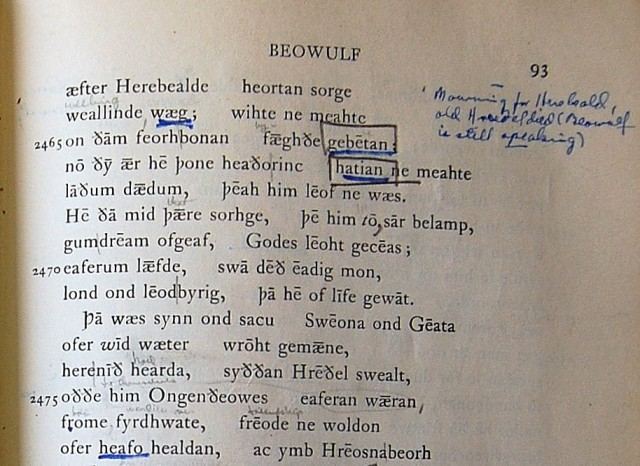
\includegraphics[width=0.8\textwidth]{beowulf}
    \caption {From squiggles to symbols}
  \end{columns}
\end{figure}
\end{frame}


\begin{frame}{Derived aptness of symbols}
\begin{figure}
  \centering
  \begin{columns}
    \column{0.99\textwidth}
    \centering
    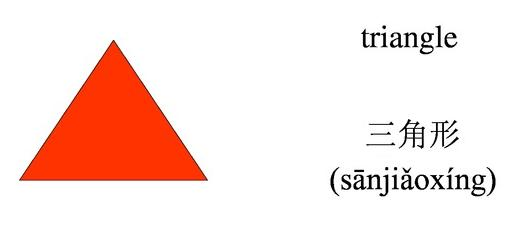
\includegraphics[width=0.8\textwidth]{triangle-chinese}
    \caption {Both convey the universal, but the shape more aptly does so.}
  \end{columns}
\end{figure}
\end{frame}


\begin{frame}[fragile]{Considerations}
  \begin{itemize}
  \item `Real' has at least two senses --- out there, and in the mind.\vspace{5mm}
  \item `Real' in the infinite mind is the primary sense, out there and then in my mind is the secondary sense (Scholastic realism).\vspace{5mm}
    \item Unity, truth and goodness are, at least in some sense, changeless. No obvious correlate for beauty can be found.
  \end{itemize}
\end{frame}


\begin{frame}[plain]
  \titlepage
\end{frame}

\end{document}
